\documentclass{classrep}
\usepackage{color}
\usepackage{url}
\usepackage{hyperref}
\usepackage{amsmath}
\usepackage[T1]{fontenc}
\usepackage{polski}
\usepackage[utf8]{inputenc}
\usepackage{graphicx}
\usepackage{upgreek}
\graphicspath{ {./rys/} }
\newtheorem{defin}{Definicja}
\usepackage{etoolbox}
\let\bbordermatrix\bordermatrix
\patchcmd{\bbordermatrix}{8.75}{4.75}{}{}
\patchcmd{\bbordermatrix}{\left(}{\left[}{}{}
\patchcmd{\bbordermatrix}{\right)}{\right]}{}{}

\studycycle{Informatyka, studia dzienne, I st.}
\coursesemester{VI}

\coursename{Komputerowe systemy rozpoznawania}
\courseyear{2019/2020}

\courseteacher{dr inż. Marcin Kacprowicz}
\coursegroup{poniedziałek, 12:00}

\author{
	\studentinfo{Radosław Grela}{216769} \and
	\studentinfo{Jakub Wąchała}{216914} 
}

\title{Zadanie 2: Lingwistyczne podsumowania baz danych}


\begin{document}
	\maketitle
	
	\section{Cel} % Cel
	Celem zadania jest stworzenie aplikacji desktopowej, która ma za zadanie generować pewną ilość podsumowań lingwistycznych dla danej bazy danych. Aplikacja musiała umożliwić automatyczne generowanie podsumowań lingwistycznych służących do tworzenia wiadomości tekstowych na podstawie dużej bazy danych (ponad 10 tyś rekordów). \cite{tresc}
	
	\section{Wprowadzenie} % Wprowadzenie
	W ramach projektu zajmowaliśmy się analizą działania lingwistycznych podsumowań baz danych na zbiorach rozmytych. Definicja zbioru rozmytego jest istotna w naszym zadaniu i brzmi następująco:
	\begin{defin}
		\label{rozmyty}
		Zbiór rozmyty A opisany na przestrzeni rozważań $\mathcal{X}$ jest zdefiniowany jako:
		\begin{equation}
		A = \{\langle x,\, \mu_A(x)\rangle : x \in \mathcal{X} \}, 
		\end{equation}
		gdzie $\mu_A: \mathcal{X} \to [0,1]$ nazywamy funkcją przynależności do zbioru rozmytego A. Jego wartość $x \in \mathcal{X}$ jest określany jako stopień przynależności x do A. \cite{anbook}
	\end{defin}

	Funkcja przynależności określa, w jakim stopniu element x przynależy do zbioru. W zbiorach rozmytych są to wartości z przedziału [0,1]. 
	
	Aby wygenerować podsumowania lingwistyczne bazy danych korzystamy z podsumowań lingwistycznych jednopodmiotowych w pierwszej i drugiej formie oraz wielopodmiotowych w pierwszych cztereach formach.
	
	\subsection{Podsumowania jednopodmiotowe w pierwszej formie  \cite{anbook}}
	Podsumowanie lingwistyczne jednopodmiotowe w pierwszej formie ma postać:
	\begin{equation}
	Q\:P\:jest\:S_j\:[T]
	\end{equation}
	gdzie
	\begin{itemize}
		\item Q - kwantyfikator absolutny lub względny, reprezentowany przez zbiór rozmyty
		\item P - podmiot podsumowania
		\item $S_j$ - sumaryzator reprezentowany przez zbiór rozmyty
		\item T - miara jakości dla podsumowania.
	\end{itemize}

	Ponadto, takie podsumowanie może mieć również postać ze złożonym sumaryzatorem:
	\begin{equation}
	Q\:P\:jest\:S_1\:AND\:S_2\:AND\ldots\:AND\:S_n[T]
	\end{equation}
	
	\subsection{Podsumowania jednopodmiotowe w drugiej formie \cite{anbook}}	
	Podsumowanie lingwistyczne jednopodmiotowe w pierwszej formie ma postać:
	\begin{equation}
	Q \: P \: \hbox{będących} \: W \: jest\:S_j\:[T]
	\end{equation}
	gdzie
	\begin{itemize}
		\item W - kwalifikator wyrażony zbiorem rozmytym.
	\end{itemize}

	Podobnie, jak w przypadku zdań jednopodmiotowych w pierwszej formie, kwalifikator moze być złożony z kilku zbiorów rozmytych oraz jednocześnie sumaryzator.
	\subsection{Podsumowania wielopodmiotowe \cite{anbookpl}}
	W podsumowaniach wielopodmiotowych przyjmuje się następujące oznaczenia:
	\begin{itemize}
		\item $P_1$, $P_2$ - podmioty podsumowań reprezentowane przez rozłączne podzbiory $\mathcal{D}_1$, $\mathcal{D}_2$ w $\mathcal{D}$
		\item $M_1$, $M_2$ - liczby obiektów w $P_1$, $P_2$
		\item Q - względny kwantyfikator lingwistyczny
		\item S i W - odpowiednio sumaryzator i kwalifikator lingwistyczny 
	\end{itemize} 
	
	Pierwsza postać podsumowań wielopodmiotowych ma postać:
	\begin{equation}
	Q \: P_1 \hbox{ w porównaniu do }P_2 \: jest\:S.
	\end{equation}
    
	Druga postać podsumowań wielopodmiotowych ma postać:
	\begin{equation}
	Q \: P_1 \hbox{ w porównaniu do tych } P_2,\hbox{ które są W, jest S.}
	\end{equation}

	Trzecia postać podsumowań wielopodmiotowych ma postać:
	\begin{equation}
	Q \:  P_1, \hbox{ które są W, w porównaniu do } P_2,\hbox{  jest S. }
	\end{equation}
	
	Czwarta postać podsumowań wielopodmiotowych ma postać:
	\begin{equation}
	\hbox{Więcej $P_1$ niż $P_2$ jest S. }
	\end{equation}
	
	\subsection{Funkcje prynależności}
	W naszym programie wykorzystujemy 3 funkcje przynależności: trapezoidalna, trójkątna oraz gaussowska.
	
	\subsubsection{Funkcja trapezoidalna}
	Funkcja trapezoidalna przyjmuje 4 parametry a, b, c, d, dla których spełniony jest warunek a $\leq$ b $\leq$ c $\leq$ d. Jej wzór jest następujący \cite{anbook}: 
	
	\begin{equation}
	\mu_A(x) = \begin{cases}
	\frac{x-a}{b-a} & \mbox{gdy } x \in (a,\, b), \\
	1                 & \mbox{gdy } x \in [b,\, c], \\
	\frac{d-x}{d-c} & \mbox{gdy } x \in (c,\, d), \\
	0                 & \mbox{w przeciwnym razie}.
	\end{cases}
	\end{equation}
	
	
	\subsubsection{Funkcja trójkątna}
	Funkcja trójkątna jest szczególnym przypadkiem funkcji trapezoidalnej. Przyjmuje ona trzy parametry a, b, c, dla których zachodzi warunek a $\leq$ b $\leq$ c. Te parametry określają punkty ,,załamania'' tej funkcji. Jej wzór jest następujący \cite{funkcje}: 
	\begin{equation}
	\mu_A(x) = \begin{cases}
	\frac{x-a}{b-a} & \mbox{gdy } x \in (a,\, b), \\
	1                 & \mbox{gdy } x = b, \\
	\frac{c-x}{c-b} & \mbox{gdy } x \in (b,\, c), \\
	0                 & \mbox{w przeciwnym razie}.
	\end{cases}
	\end{equation}
	
	
	
	
	\subsubsection{Funkcja Gaussowska} 
	Funkcja Gaussowska jest definiowana przez 2 parametry które określają środek funkcji oraz jej szerokość. Wzór jest następujący \cite{kul}:
	\begin{equation}
		\mu_A(x) = e^{(-(\frac{x - \bar{x}}{\sigma})^2)}
	\end{equation}
	gdzie 
	\begin{itemize}
		\item $\bar{x}$ jest środkiem funkcji,
		\item $\sigma$ określa szerokość krzywej Gaussowskiej. 
	\end{itemize}
	
	\section{Miary jakości}
	\subsection{Miary jakości dla zdań jednopodmiotowych}
	\subsubsection{Degree of truth}
\textsl{Degree of truth} to suma przynależności wszystkich rozważanych krotek do podsumowania lingwistycznego. Dla zdań jednopodmiotowych bez kwalifikatora oraz kwantyfikatorów relatywnych wzór wygląda następująco:
	\begin{equation}
	T_1 = \mu_Q(\frac{r}{m})
	\end{equation}
natomiast zdań jednopodmiotowych bez kwalifikatora oraz kwantyfikatorów absolutnych:
	\begin{equation}
	T_1 = \mu_Q(r)
	\end{equation}
gdzie 
	\begin{equation}
r = \sum_{i=1}^{m} \mu_{S} (d_i)
	\end{equation}
a $m$ to liczba krotek w bazie danych.

Dla zdań jednopodmiotowych z kwalifikatorem kwantyfikator może być tylko względny, a wzór wygląda następująco:
\begin{equation}
T_1 = \mu_Q(r)
\end{equation}
gdzie 
\begin{equation}
r = \frac{\sum_{i=1}^{m} (\mu_{S} (d_i) \land \mu_{W} (d_i))}{\sum_{i=1}^{m} \mu_{W} (d_i)}
\end{equation}

	\subsubsection{Degree of imprecision}
\textsl{Degree of imprecision} określa stopień precyzyjności sumaryzatora. Dany jest wzorem:
	\begin{equation}
T_2 = 1 - \left(\prod_{j=1}^{n} \mathrm{in}(S_j)\right)^{1/n}
	\end{equation}
gdzie $in(S_j)$ to stopień rozmycia wyrażony wzorem
$
in(s_j) = \frac{|supp(S_j)|}{|X|}
$
a z kolei $supp(\cdot)$ oznacza nośnik zbioru rozmytego.


	\subsubsection{Degree of covering}
\textsl{Degree of covering} reprezentuje, stopień, w jakim nośnik sumaryzatora pokrywa się z nośnikiem kwalifikatora. Dany jest wzorem:
	\begin{equation}
T_3 = \frac{\sum_{i=1}^{m}t_i}{\sum_{i=1}^{m}h_i}
	\end{equation}
gdzie dla zdań z kwalifikatorem:
\[
\begin{array}{l}
t_i = \begin{cases}
1 & \mbox{gdy } \mu_{S}(d_i) > 0 ~ \wedge ~ \mu_{W}(d_i) > 0 \\
0 & \mbox{w przeciwnym razie.}
\end{cases} \\
h_i = \begin{cases}
1 & \mbox{gdy } \mu_{W}(d_i) > 0 \\
0 & \mbox{w przeciwnym razie.}
\end{cases}
\end{array}\]
a dla zdań bez kwalifikatora:
\[
\begin{array}{l}
t_i = \begin{cases}
1 & \mbox{gdy } \mu_{S}(d_i) > 0  \\
0 & \mbox{w przeciwnym razie.}
\end{cases} \\
\end{array}\]
\[h_i = 1\]



	\subsubsection{Degree of appropriateness}
\textsl{Degree of appropriateness} definiuje, jak dużo krotek przynależy do sumaryzatora, czyli czy określone podsumowanie jest odpowiednie dla zestawu danych. Dany jest wzorem:
\begin{equation}
T_4 = \left| \prod_{j=1}^{n} r_j - T_3\right|
\end{equation}
gdzie
\begin{equation}
r_j = \frac{\sum_{i=1}^{m} g_{ij}}{m}
\end{equation}
natomiast
$
g_{ij} = \begin{cases}
1 & \mbox{gdy } \mu_{S_j}(d_i) > 0 \\
0 & \mbox{w przeciwnym wypadku.}
\end{cases}
$


	\subsubsection{Length of a summary}
\textsl{Length of a summary}  określa jakość podsumowania na podstawie złożoności sumaryzatora, czyli im więcej składowych sumaryzatora złożonego, ty niższa wartość tej miary. Dany jest wzorem:
\begin{equation}
T_5 = 2 \cdot \left( \frac{1}{2}\right)^{|S|} 
\end{equation}
gdzie $|S|$ to liczba zbiorów rozmytych z jakich złożony jest sumaryzator.


	\subsubsection{Degree of quantifier imprecision}
\textsl{Degree of quantifier imprecision} przedstawia w jakim stopniu precyzyjny jest kwantyfikator. Im mniejszy nośnik zbioru rozmytego  tym wyższa jest jego precyzja. Dany jest wzorem:
\begin{equation}
T_6 = 1 - in(Q) = 1 - \frac{|supp(Q)|}{|\mathcal{X}_Q|}
\end{equation}
gdzie $|\mathcal{X}_Q| = 1$ dla kwantyfikatora relatywnego, natomiast dla kwantyfikatora absolutnego $|\mathcal{X}_Q| = m$, czyli liczba krotek w bazie danych.


	\subsubsection{Degree of quantifier cardinality}
\textsl{Degree of quantifier cardinality} opisuje stopień precyzji kwantyfikatora, im większa kardynalność kwantyfikatora tym jest on mniej precyzyjny. Dany jest wzorem:
\begin{equation}
T_7 = 1 - \frac{|Q|}{|\mathcal{X}_Q|}
\end{equation}
gdzie $|\cdot| = clm(\cdot)$ - całka z funkcji przynależności zbioru rozmytego (czyli pole pod jego wykresem).


	\subsubsection{Degree of summarizer cardinality}
\textsl{Degree of summarizer cardinality} opisuje stopień precyzji sumaryzatora, im mniejsza kardynalność sumaryzatora tym jest on bardziej przecyzyjny. Dany jest wzorem:
\begin{equation}
T_8 = 1- \left(\prod_{j=1}^{n} \frac{|S_j|}{|\mathcal{X}_j|}\right)^{\frac{1}{n}}
\end{equation}
gdzie $n$ to liczba zbiorów rozmytych z jakich stworzony jest sumaryzator.


	\subsubsection{Degree of qualifier imprecision}
\textsl{Degree of qualifier imprecision} określa, w jakim stopniu precyzyjny jest kwalifikator. Im szerszy nośnik zbioru rozmytego tym niższa jest jego precyzja. Dany jest wzorem:
\begin{equation}
T_{9} = 1 - \left(\prod_{j=1}^{x} in(W_{gj})\right)^{\frac{1}{x}}
\end{equation}
gdzie $in(W_{gj})$ to stopień rozmycia zbioru rozmytego $W_{gj}$.


	\subsubsection{Degree of qualifier cardinality}
\textsl{Degree of qualifier cardinality} opisuje stopień precyzji kwalifikatora, im większa jest kardynalność kwalifikatora, tym jest on mniej precyzyjny. Dany jest wzorem:
\begin{equation}
T_{10} = 1- \left(\prod_{j=1}^{x} \frac{|W_{gj}|}{|\mathcal{X}_{gj}|}\right)^{\frac{1}{x}}
\end{equation}


	\subsubsection{Length of qualifier}
\textsl{Length of qualifier} wyznacza jakość podsumowania na podstawie złożoności kwalifikatora. Im bardziej złożony kwalifikator, tym jakość podsumowania jest gorsza. Dany jest wzorem:
\begin{equation}
T_{11} = 2 \cdot \left(\frac{1}{2}\right)^{|W|}
\end{equation}
gdzie $|W|$ to liczba zbiorów rozmytych, z jakich stworzony jest kwalifikator.

\subsection{Miary jakości dla zdań wielopodmiotowych}
Dla zdań wielopodmiotowych liczymy tylko stopień prawdziwości, czyli miarę $T_1$.

\subsubsection{Degree of truth dla zdań wielopodmiotowych w pierwszej formie \cite{anarticle30}} 
\begin{equation}
T_{1_1} = \left(\frac{\frac{1}{M_1} \Upsigma-count(S_{P1})}
				{\frac{1}{M_1} \Upsigma-count(S_{P1}) + \frac{1}{M_2} \Upsigma-count(S_{P2})}\right)
\end{equation}
gdzie 
\begin{itemize}
	\item $\Upsigma-count(S_{P1}) = \sum_{i=1}^{m} \{\mu_{S}(d_i) : d_i \in^* P_1\}$
	\item $\Upsigma-count(S_{P2}) = \sum_{i=1}^{m} \{\mu_{S}(d_i) : d_i \in^* P_2\}$
	\item $M_1$ to liczba krotek reprezentujących podmiot $P_1$
	\item $M_2$ to liczba krotek reprezentujących podmiot $P_2$
\end{itemize}
\subsubsection{Degree of truth dla zdań wielopodmiotowych w drugiej formie \cite{anbookpl}} 
\begin{equation}
T_{1_2} = \left(\frac{\frac{1}{M_1} \Upsigma-count(S_{P1})}
				{\frac{1}{M_1} \Upsigma-count(S_{P1}) + \frac{1}{M_2} \Upsigma-count(S_{P2} \cap W )}\right)
\end{equation}
gdzie 
\begin{itemize}
	\item  $\Upsigma-count(S_{P2} \cap W ) = \sum_{i=1}^{m} \{min(\mu_{S1}(d_i), \mu_{W}(d_i)) : d_i \in^* P_2 \}  $
\end{itemize}
\subsubsection{Degree of truth dla zdań wielopodmiotowych w trzeciej formie \cite{anbookpl}} 
\begin{equation}
T_{1_3} = \left(\frac{\frac{1}{M_1} \Upsigma-count(S_{P1} \cap W)}
				{\frac{1}{M_1} \Upsigma-count(S_{P1} \cap W) + \frac{1}{M_2} \Upsigma-count(S_{P2} )}\right)
\end{equation}
gdzie 
\begin{itemize}
	\item  $\Upsigma-count(S_{P1} \cap W ) = \sum_{i=1}^{m} \{min(\mu_{S1}(d_i), \mu_{W}(d_i)) : d_i \in^* P_1 \}  $
\end{itemize}
\subsubsection{Degree of truth dla zdań wielopodmiotowych w czwartej formie \cite{anarticle30}} 
\begin{equation}
T_{1_3} = \left(\frac{\Upsigma-count(S_{P1})}
			{\Upsigma-count(S_{P1}) + \Upsigma-count(S_{P2})}\right)
\end{equation}


	\newpage
	\section{Opis implementacji} % Opis implementacji
	Program został stworzony w języku C\#. Graficzny interfejs użytkownika został stworzony przy wykorzystaniu Windows Presentation Foundation. Poniżej przedstawiamy uproszczony diagram UML naszego programu.
	
	\begin{figure}[h!]
		\centering
		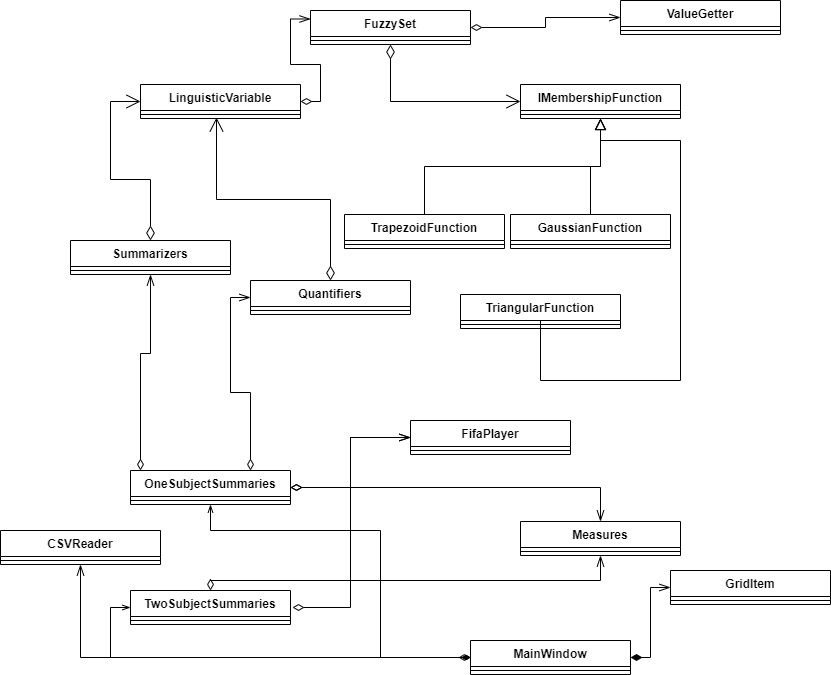
\includegraphics[width=0.9\textwidth]{../uml/uml.png}
		\caption{Diagram UML.}
		\label{uml}
	\end{figure}
	
	\begin{itemize}
		\item Klasa Summarizers przechowuje poszczególne sumaryzatory, np "młody", "wysoki" 
		\item Quantifiers jest klasą odpowiedzialną za kwantyfikatory relatywne oraz absolutne
		\item CSVReader odpowiada za wczytanie pliku csv z danymi do programu
		\item FuzzySet to klasa odpowiadająca za zbiór rozmyty
		\item Klasy TrapezoidFunction, GaussianFunction, TriangularFunction odpowiadają za odpowiednie funkcje przynależności
		\item FifaPlayer to klasa, która reprezentuje krotkę bazy danych
		\item LinguisticVariable to klasa reprezentująca zmienną lingwistyczną.
	\end{itemize}
	
	\section{Materiały i metody} % Materiały i metody
	\subsection{Baza danych}
	Do przeprowadzania badań oraz do generowania podsumowań wykorzystaliśmy bazę danych dotyczącą piłkarzy z gry FIFA 20. Pochodzi ona ze źródła \cite{baza}. Składa się ona z 18278 rekordów posiadających 104 atrybuty. Do naszego projektu skorzystamy z 11. Są to następujące atrybuty:
	
	\begin{enumerate}
		\item Wiek - \textsl{age} - wartość z przedziału [16, 42]
		\item Wzrost (w cm) - \textsl{height\_cm} - wartość z przedziału [156, 205]
		\item Waga (w kg) - \textsl{weight\_kg} - wartość z przedziału [50, 110]
		\item Ocena ogólna - \textsl{overall} - wartość z przedziału [48, 94]
		\item Wykończenie - \textsl{attacking\_finishing} - wartość z przedziału [2, 95]
		\item Dribbling - \textsl{skill\_dribbling} - wartość z przedziału [4, 97]
		\item Podkręcenie piłki - \textsl{skill\_curve} - wartość z przedziału [6, 94]
		\item Długie podania - \textsl{skill\_long\_passing} - wartość z przedziału [8, 92]
		\item Sprint - \textsl{movement\_sprint\_speed} - wartość z przedziału [11, 96]
		\item Siła strzału - \textsl{power\_shot\_power} - wartość z przedziału [14, 95]
	\end{enumerate}

	Każda z kolumn jest typu całkowitego.

	\subsection{Zmienne lingwistyczne}
	% wiek -------------------------------
	\subsubsection{Wiek}
	Należy zauważyć, że wiek w przypadku zawodnika piłki nożnej oceniany jest w inny sposób niż wiek przeciętnego człowieka.
	\begin{itemize}
		\item \textsl{(16-21) bardzo młody}
		\item \textsl{(20-25) młody}
		\item \textsl{(24-32) średni}
		\item \textsl{(31-42) stary}
	\end{itemize}
	
	\begin{table}[h!]
		\centering
		\begin{tabular} {c c c c c}
			\hline
			\textbf{Etykieta} & \textbf{a} & \textbf{b} & \textbf{c} & \textbf{d} \\ [0.5ex] 
			\hline	
			\hline 
			bardzo młody & 16 & 16 & 18 & 21  \\
			młody & 20 & 22 & 24 & 25  \\
			średni & 24 & 26 & 29 & 32  \\
			stary & 31 & 34 & 42 & 42  \\
			\hline
		\end{tabular}
		\caption{Przyporządkowane parametry funkcji trapezoidalnej dla atrybutu  Wiek. }
		\label{tabelaWiek}
	\end{table}

	\begin{figure}[h!]
		\centering
		\includegraphics[width=0.9\textwidth]{zmienne/1.png}
		\caption{Funkcja przynależności (trapezoidalna) dla atrybutu Wiek.}
		\label{wykresWiek}
	\end{figure}
	
	% wzrost ---------------------------
	\newpage
	\subsubsection{Wzrost}
	\begin{itemize}
		\item \textsl{(156-166) niski}
		\item \textsl{(164-177) średni}
		\item \textsl{(175-188) wysoki}
		\item \textsl{(186-205) bardzo wysoki}
	\end{itemize}
	
	\begin{table}[h!]
		\centering
		\begin{tabular} {c c c c}
			\hline
			\textbf{Etykieta} & \textbf{a} & \textbf{b} & \textbf{c} \\ [0.5ex] 
			\hline	
			\hline 
			niski & 156 & 156 & 166 \\
			średni & 164 & 170 & 177 \\
			wysoki & 175 & 182 & 188 \\
			bardzo wysoki & 186 & 205 & 205  \\
			\hline
		\end{tabular}
		\caption{Przyporządkowane parametry funkcji trójkątnej dla atrybutu Wzrost. }
		\label{tabelaWzrost}
	\end{table}
	
	\begin{figure}[h!]
		\centering
		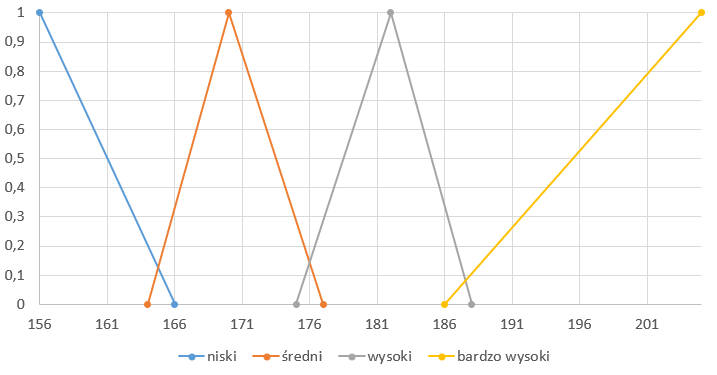
\includegraphics[width=0.9\textwidth]{zmienne/2.png}
		\caption{Funkcja przynależności (trapezoidalna) dla atrybutu Wzrost.}
		\label{wykresWzrost}
	\end{figure}

	% waga ---------------------------
	\newpage
	\subsubsection{Waga}
	\begin{itemize}
		\item \textsl{(50-65) bardzo chudy}
		\item \textsl{(55-85) chudy}
		\item \textsl{(75-105) średni}
		\item \textsl{(95-110) gruby}
	\end{itemize}
	
	\begin{table}[h!]
		\centering
		\begin{tabular} {c c c}
			\hline
			\textbf{Etykieta} & \textbf{$\bar{x}$} & \textbf{$\sigma$} \\ [0.5ex] 
			\hline	
			\hline 
			bardzo chudy & 50 & 8  \\
			chudy & 70 & 8  \\
			średni & 90 & 8  \\
			gruby & 110 & 8  \\
			\hline
		\end{tabular}
		\caption{Przyporządkowane parametry funkcji gaussowskiej dla atrybutu  Waga. }
		\label{tabelaWaga}
	\end{table}
	
	\begin{figure}[h!]
		\centering
		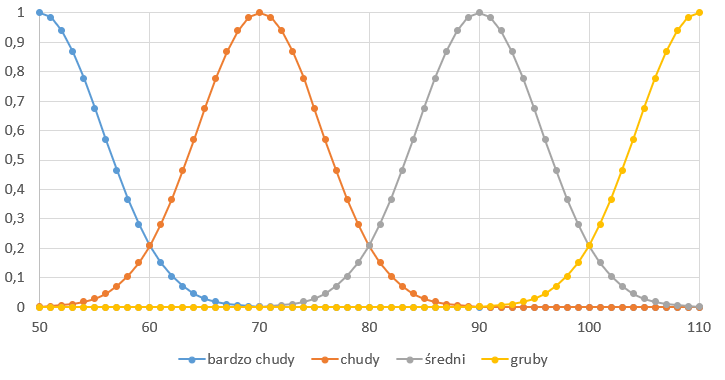
\includegraphics[width=0.9\textwidth]{zmienne/3.png}
		\caption{Funkcja przynależności (gaussowska) dla atrybutu Waga.}
		\label{wykresWaga}
	\end{figure}
	
	% Ocena ogólna -------------------------------
	\newpage
	\subsubsection{Ocena ogólna}
	\begin{itemize}
		\item \textsl{(48-65) słaby}
		\item \textsl{(60-75) średni}
		\item \textsl{(70-87) dobry}
		\item \textsl{(85-94) bardzo dobry}
	\end{itemize}
	
	\begin{table}[h!]
		\centering
		\begin{tabular} {c c c c c}
			\hline
			\textbf{Etykieta} & \textbf{a} & \textbf{b} & \textbf{c} & \textbf{d} \\ [0.5ex] 
			\hline	
			\hline 
			słaby & 48 & 48 & 59 & 65  \\
			średni & 60 & 65 & 70 & 75  \\
			dobry & 70 & 78 & 85 & 87  \\
			bardzo dobry & 85 & 90 & 94 & 94  \\
			\hline
		\end{tabular}
		\caption{Przyporządkowane parametry funkcji trapezoidalnej dla atrybutu  Ocena ogólna. }
		\label{tabelaOverall}
	\end{table}
	
	\begin{figure}[h!]
		\centering
		\includegraphics[width=0.9\textwidth]{zmienne/4.png}
		\caption{Funkcja przynależności (trapezoidalna) dla atrybutu Ocena ogólna.}
		\label{wykresOverall}
	\end{figure}
	
	
	% Wykończenie -------------------------------
	\newpage
	\subsubsection{Wykończenie}
	\begin{itemize}
		\item \textsl{(2-35) bardzo słabe}
		\item \textsl{(30-60) słabe}
		\item \textsl{(50-80) średnie}
		\item \textsl{(75-87) dobre}
		\item \textsl{(85-95) bardzo dobre}
	\end{itemize}
	
	\begin{table}[h!]
		\centering
		\begin{tabular} {c c c c c}
			\hline
			\textbf{Etykieta} & \textbf{a} & \textbf{b} & \textbf{c} & \textbf{d} \\ [0.5ex] 
			\hline	
			\hline 
			bardzo słabe & 2 & 2 & 25 & 35  \\
			słabe & 30 & 35 & 50 & 60  \\
			średnie & 50 & 55 & 75 & 80  \\
			dobre & 75 & 80 & 85 & 87  \\
			bardzo dobre & 85 & 90 & 95 & 95  \\			
			\hline
		\end{tabular}
		\caption{Przyporządkowane parametry funkcji trapezoidalnej dla atrybutu  Wykończenie. }
		\label{tabelaWykonczenie}
	\end{table}
	
	\begin{figure}[h!]
		\centering
		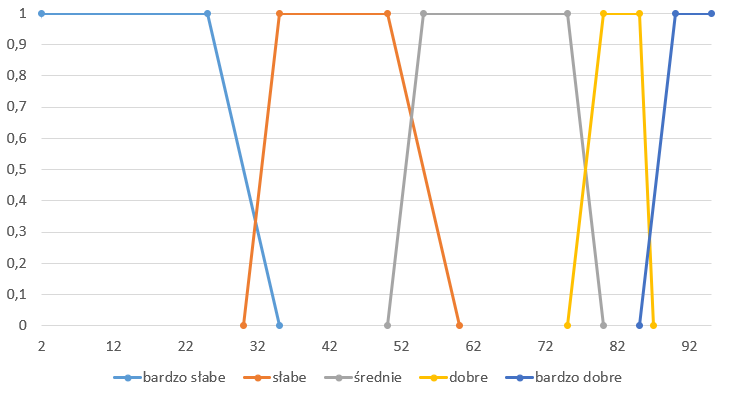
\includegraphics[width=0.9\textwidth]{zmienne/5.png}
		\caption{Funkcja przynależności (trapezoidalna) dla atrybutu Wykończenie.}
		\label{wykresWykonczenie}
	\end{figure}

	
	% Dribbling -------------------------------
	\newpage
	\subsubsection{Dribbling}
	\begin{itemize}
		\item \textsl{(4-35) bardzo słaby}
		\item \textsl{(30-60) słaby}
		\item \textsl{(50-70) średni}
		\item \textsl{(68-87) dobry}
		\item \textsl{(85-97) bardzo dobry}
	\end{itemize}
	
	\begin{table}[h!]
		\centering
		\begin{tabular} {c c c c c}
			\hline
			\textbf{Etykieta} & \textbf{a} & \textbf{b} & \textbf{c} & \textbf{d} \\ [0.5ex] 
			\hline	
			\hline 
			bardzo słaby & 4 & 4 & 25 &	35 \\
			słaby & 30 & 35 & 50 & 60  \\
			średni & 50 & 55 & 68 & 70  \\
			dobry & 68 & 73 & 85 & 87  \\
			bardzo dobry & 85 & 90 & 97 & 97  \\		
			\hline
		\end{tabular}
		\caption{Przyporządkowane parametry funkcji trapezoidalnej dla atrybutu Dribbling. }
		\label{tabelaDribbling}
	\end{table}
	
	\begin{figure}[h!]
		\centering
		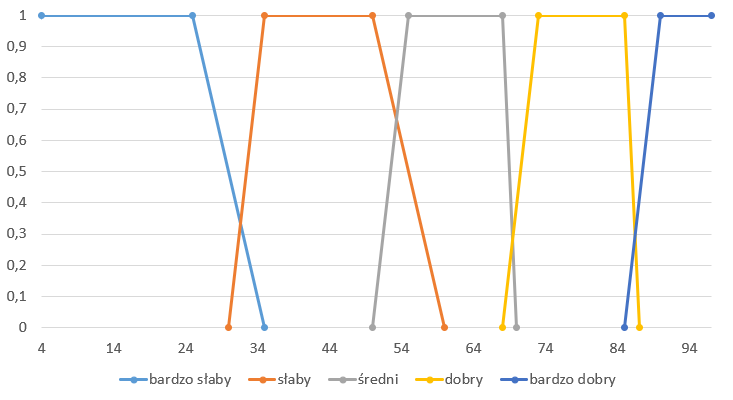
\includegraphics[width=0.9\textwidth]{zmienne/6.png}
		\caption{Funkcja przynależności (trapezoidalna) dla atrybutu Dribbling.}
		\label{wykresDribbling}
	\end{figure}
	
	
	% Podkręcenie piłki -------------------------------
	\newpage
	\subsubsection{Podkręcenie piłki}
	\begin{itemize}
		\item \textsl{(6-35) bardzo słabe}
		\item \textsl{(30-60) słabe}
		\item \textsl{(50-70) średnie}
		\item \textsl{(68-87) dobre}
		\item \textsl{(85-94) bardzo dobre}
	\end{itemize}
	
	\begin{table}[h!]
		\centering
		\begin{tabular} {c c c c}
			\hline
			\textbf{Etykieta} & \textbf{a} & \textbf{b} & \textbf{c} \\ [0.5ex] 
			\hline	
			\hline 
			bardzo słabe & 6 & 6 & 35 \\
			słabe & 20 & 35 & 60   \\
			średnie & 50 & 60 & 70  \\
			dobre & 68 & 75 & 87   \\
			bardzo dobre & 85 & 94 & 94  \\					
			\hline
		\end{tabular}
		\caption{Przyporządkowane parametry funkcji trójkątnej dla atrybutu Podkręcenie piłki. }
		\label{tabelaPodkrecenie}
	\end{table}
	
	\begin{figure}[h!]
		\centering
		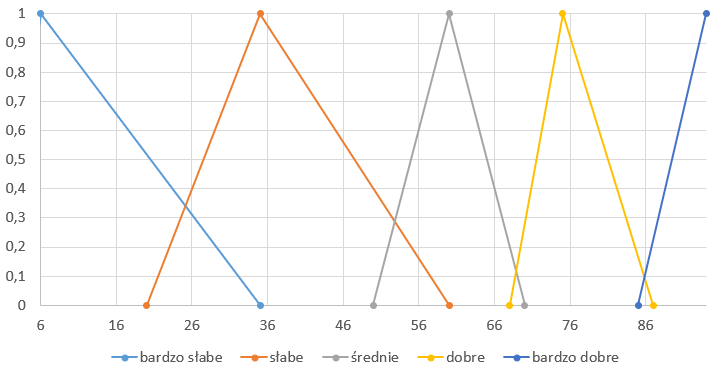
\includegraphics[width=0.9\textwidth]{zmienne/7.png}
		\caption{Funkcja przynależności (trójkątna) dla atrybutu Podkręcenie piłki.}
		\label{wykresPodkrecenie}
	\end{figure}
	
	
	% Długie podania -------------------------------
	\newpage
	\subsubsection{Długie podania}
	\begin{itemize}
		\item \textsl{(8-35) bardzo słabe}
		\item \textsl{(30-60) słabe}
		\item \textsl{(50-70) średnie}
		\item \textsl{(68-85) dobre}
		\item \textsl{(82-92) bardzo dobre}
	\end{itemize}
	\begin{table}[h!]
		\centering
		\begin{tabular} {c c c c c}
			\hline
			\textbf{Etykieta} & \textbf{a} & \textbf{b} & \textbf{c} & \textbf{d} \\ [0.5ex] 
			\hline	
			\hline 
			bardzo słabe & 8 & 8 & 25 &	35 \\
			słabe & 30 & 35 & 50 & 60  \\
			średnie & 50 & 55 & 68 & 70  \\
			dobre & 68 & 73 & 80 & 85  \\
			bardzo dobre & 82 & 85 & 92 & 92  \\	
			\hline
		\end{tabular}
		\caption{Przyporządkowane parametry funkcji trapezoidalnej dla atrybutu Długie podania. }
		\label{tabelaPodania}
	\end{table}
	\begin{figure}[h!]
		\centering
		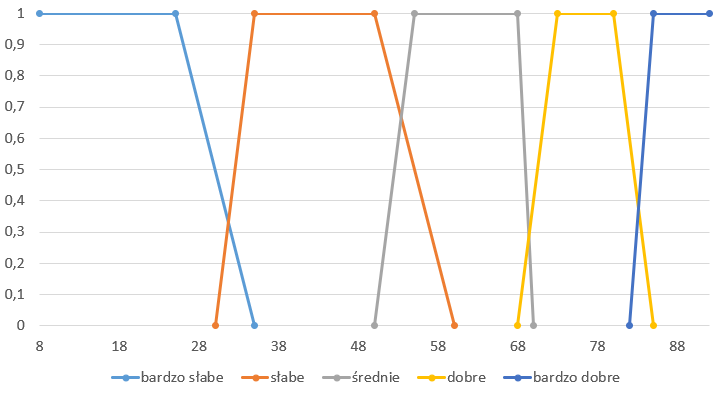
\includegraphics[width=0.9\textwidth]{zmienne/8.png}
		\caption{Funkcja przynależności (trapezoidalna) dla atrybutu Długie podania.}
		\label{wykresPodania}
	\end{figure}

	% Sprint -------------------------------
	\newpage
	\subsubsection{Sprint}
	\begin{itemize}
		\item \textsl{(11-35) bardzo wolny}
		\item \textsl{(30-55) wolny}
		\item \textsl{(50-70) średni}
		\item \textsl{(68-86) szybki}
		\item \textsl{(84-96) bardzo szybki}
	\end{itemize}
	\begin{table}[h!]
		\centering
		\begin{tabular} {c c c c c}
			\hline
			\textbf{Etykieta} & \textbf{a} & \textbf{b} & \textbf{c} & \textbf{d} \\ [0.5ex] 
			\hline	
			\hline 
			bardzo wolny & 11 & 11 & 25 &	35 \\
			wolny & 30 & 35 & 48 & 55  \\
			średni & 50 & 55 & 68 & 70  \\
			szybki & 68 & 73 & 80 & 86  \\
			bardzo szybki & 84 & 90 & 96 & 96  \\	
			\hline
		\end{tabular}
		\caption{Przyporządkowane parametry funkcji trapezoidalnej dla atrybutu Sprint. }
		\label{tabelaSprint}
	\end{table}
	\begin{figure}[h!]
		\centering
		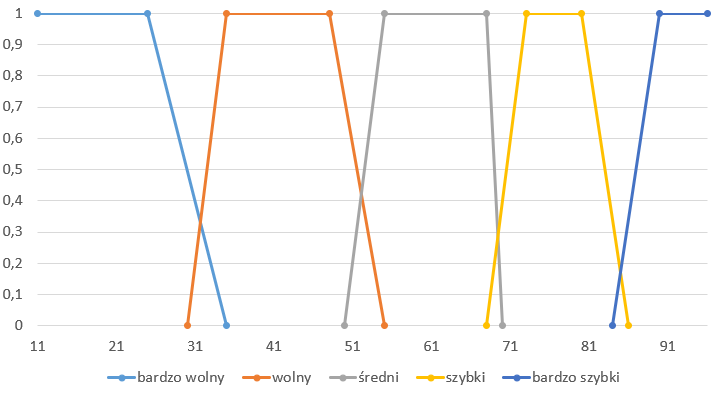
\includegraphics[width=0.9\textwidth]{zmienne/9.png}
		\caption{Funkcja przynależności (trapezoidalna) dla atrybutu Sprint.}
		\label{wykresSprint}
	\end{figure}


	% Siła strzału -------------------------------
	\newpage
	\subsubsection{Siła strzału}
	\begin{itemize}
		\item \textsl{(14-50) słaba}
		\item \textsl{(45-65) średnia}
		\item \textsl{(62-82) duża}
		\item \textsl{(80-95) bardzo duża}
	\end{itemize}
	\begin{table}[h!]
		\centering
		\begin{tabular} {c c c c c}
			\hline
			\textbf{Etykieta} & \textbf{a} & \textbf{b} & \textbf{c} & \textbf{d} \\ [0.5ex] 
			\hline	
			\hline 
			słaba & 14 & 14 & 45 & 50 \\
			średnia & 45 & 50 & 60 & 65  \\
			duża & 62 & 68 & 80 & 82  \\
			bardzo duża & 80 & 88 & 95 & 95  \\			
			\hline
		\end{tabular}
		\caption{Przyporządkowane parametry funkcji trapezoidalnej dla atrybutu Siła strzału. }
		\label{tabelaStrzal}
	\end{table}
	\begin{figure}[h!]
		\centering
		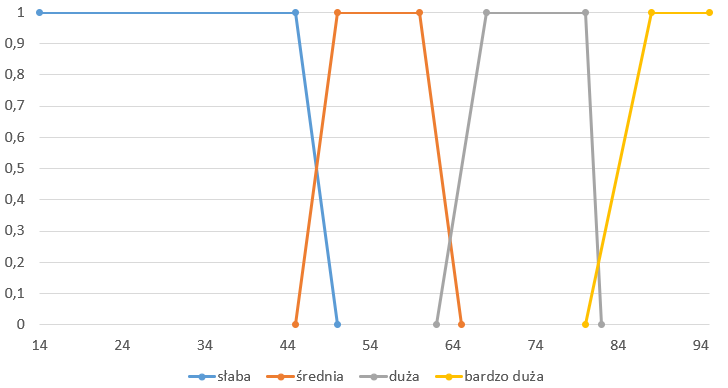
\includegraphics[width=0.9\textwidth]{zmienne/10.png}
		\caption{Funkcja przynależności (trapezoidalna) dla atrybutu Siła strzału.}
		\label{wykresStrzal}
	\end{figure}

	\newpage
	\subsection{Kwantyfikator względny}
	
	Poniżej przedstawiliśmy wartości parametrów oraz wykres funkcji przynależności dla kwantyfikatora względnego. Liczba rekordów w naszej bazie danych wynosi 18278, wykres zawiera się w wartościach [0, 1].
	\begin{table}[h!]
		\centering
		\begin{tabular} {c c c c c}
			\hline
			\textbf{Etykieta} & \textbf{a} & \textbf{b} & \textbf{c} & \textbf{d} \\ [0.5ex] 
			\hline	
			\hline 
			prawie nikt			 & 0,000 & 0,000 & 0,055 & 0,164 \\
			mniejszość			 & 0,109 & 0,164 & 0,383 & 0,438  \\
			połowa				 & 0,410 & 0,438 & 0,547 & 0,574  \\
			większość 		 	 & 0,547 & 0,602 & 0,821 & 0,875  \\	
			prawie wszyscy		 & 0,821 & 0,903 & 1,000 & 1,000  \\						
			\hline			
		\end{tabular}
		\caption{Przyporządkowane parametry funkcji trapezoidalnej dla kwantyfikatora względnego. }
		\label{tabelaKwantyfikatorWzgledny}
	\end{table}
	
	\begin{figure}[h!]
		\centering
		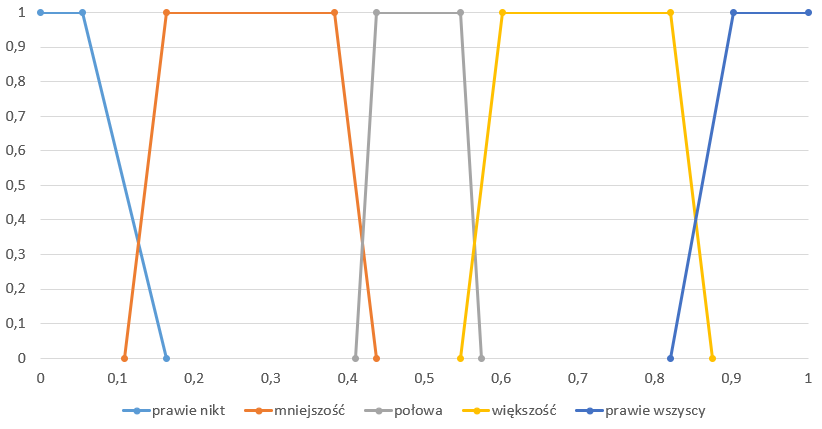
\includegraphics[width=0.9\textwidth]{kwantyfikatorWzgledny.png}
		\caption{Funkcja przynależności kwantyfikatora względnego.}
		\label{kwantyfikatorWzgledny}
	\end{figure}

	\subsection{Kwantyfikator absolutny}
	\begin{table}[h!]
		\centering
		\begin{tabular} {c c c c c}
			\hline
			\textbf{Etykieta} & \textbf{a} & \textbf{b} & \textbf{c} & \textbf{d} \\ [0.5ex] 
			\hline	
			\hline 
			Około 1000			 & 900 & 960 & 1040 & 1100 \\
			Więcej niż 3000			 & 0,109 & 0,164 & 0,383 & 0,438  \\
			Mniej niż 3000				 & 0 & 0 & 2990 & 3010  \\
			Około 500 		 	 & 450 & 480 & 520 & 550  \\	
			Około 100		 & 80 & 90 & 110 & 120  \\						
			\hline			
		\end{tabular}
		\caption{Przyporządkowane parametry funkcji trapezoidalnej dla kwantyfikatora absolutnego. }
		\label{tabelaKwantyfikatorAbsolutny}
	\end{table}
	
	\subsection{Przeprowadzone eksperymenty}
	Eksperymenty, jakie zdecydowaliśmy przedstawić są następujące:
	\begin{enumerate}
		\item Porównanie miar jakości dla różnych kwantyfikatorów w zdaniach jednopodmiotowych.
		\item Porównanie podsumowań z kwalifikatorem oraz bez (zdania jednopodmiotowe w formie pierwszej i drugiej).
		\item Porównanie podsumowań z sumaryzatorem oraz złączeniem kilku sumaryzatorów
		\item Porównanie miary degree of truth dla różnych typów zdań wielopodmiotowych.
	\end{enumerate}

	\section{Wyniki} % Wyniki
	\subsection{Porównanie miar jakości dla różnych kwantyfikatorów}
	\subsubsection{Zdania jednopodmiotowe w pierwszej formie}
	W tej części eksperymentu wygenerowaliśmy zdania dla jednego sumaryzatora "average overall".
	W tabeli oraz na wykresie poniżej zamieściliśmy tylko wyniki dla miar $T_1, T_6$ oraz $T_7$, ponieważ pozostałe miary miały stałe wyniki i wynosiły następująco: $T_2 = 0.674, T_3 = 0.684, T_4 = 0, T_5 = 1, T_8 = 0.333, T_9 = 0, T_{10} = 0, T_{11} = 0 $
	
	\begin{figure}[h!]
		\centering
		\includegraphics[width=0.9\textwidth]{ex/1.png}
		\caption{Porównanie miar jakości T1, T6 i T7 w zależności od różnych kwantyfikatorów w zdaniu jednopodmiotowym w pierwszej formie.}
		\label{wykresex1a}
	\end{figure}
\begin{table}[h!]
	\centering
	\begin{tabular} {c c c c}
		\hline
		\textbf{Kwantyfikator} & \textbf{$T_1$} & \textbf{$T_6$} & \textbf{$T_7$} \\ [0.5ex] 
		\hline	
		\hline 
		Almost none	& 0 &	0,836 &	0,89 \\
		Less	& 0	& 0,671	& 0,726 \\
		Half	& 1 &	0,836	& 0,863 \\
		Most	& 0 &	0,672	& 0,726 \\ 
		Almost all &	0&	0,821	& 0,862 \\ 
		About 1000	& 0 &	0,989	& 0,992 \\ 
		More than 3000	& 1 &	0,164 &	0,164 \\ 
		Less than 3000	& 0 &	0,835 &	0,836 \\ 
		Around 500	& 0 &	0,995	& 0,996 \\ 
		Around 100	& 0 &	0,998	& 0,998	\\ 					
		\hline			
	\end{tabular}
	\caption{Miary $T_1$, $T_6$ oraz $T_7$ dla różnych kwantyfikatorów. }
	\label{tabelaex1}
\end{table}
	\newpage
	\subsubsection{Zdania jednopodmiotowe w drugiej formie}	
	W tej części eksperymentu wygenerowaliśmy zdania dla jednego sumaryzatora "average curve" oraz kwalifikatora "good long passing".
	W tabeli oraz na wykresie poniżej zamieściliśmy tylko wyniki dla miar $T_1, T_6$ oraz $T_7$, ponieważ pozostałe miary miały stałe wyniki i wynosiły następująco: $T_2 = 0.773, T_3 = 0.431, T_4 = 0.073, T_5 = 1, T_8 = 0.5, T_9 = 0.798, T_{10} = 0.294, T_{11} = 1$
	
	\begin{figure}[h!]
		\centering
		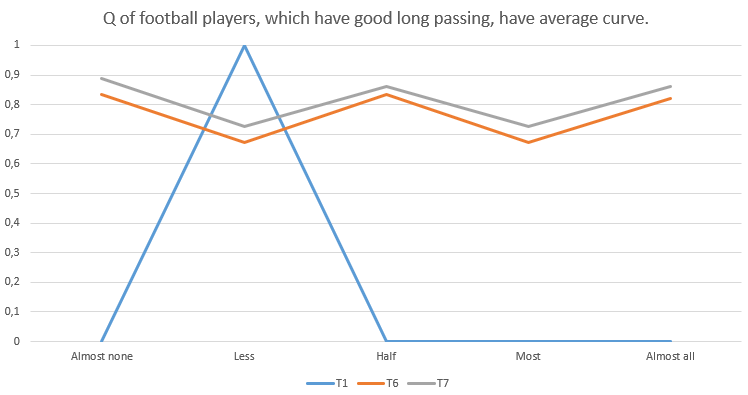
\includegraphics[width=0.9\textwidth]{ex/1b.png}
		\caption{Porównanie miar jakości T1, T6 i T7 w zależności od różnych kwantyfikatorów w zdaniu jednopodmiotowym w drugiej formie.}
		\label{wykresex1b}
	\end{figure}
	
	\begin{table}[h!]
		\centering
		\begin{tabular} {c c c c}
			\hline
			\textbf{Kwantyfikator} & \textbf{$T_1$} & \textbf{$T_6$} & \textbf{$T_7$} \\ [0.5ex] 
			\hline	
			\hline 
			Almost none	& 0 &	0,836 &	0,89 \\
			Less	& 0	& 0,671	& 0,726 \\
			Half	& 1 &	0,836	& 0,863 \\
			Most	& 0 &	0,672	& 0,726 \\ 
			Almost all & 0 &	0,821	& 0,862 \\ 				
			\hline			
		\end{tabular}
		\caption{Miary $T_1$, $T_6$ oraz $T_7$ dla różnych kwantyfikatorów. }
		\label{tabelaex1b}
	\end{table}
	
	\newpage
	\subsection{Porównanie podsumowań z kwalifikatorem oraz bez}
	W tym eksperymencie sprawdziliśmy, jak kwalifikator wpływa na jakość wyników w zdaniach jednopodmiotowych w drugiej formie. Porównania dokonaliśmy na dwóch różnych przypadkach.
	
	W pierwszym przypadku, kwantyfikatorem była etykieta "Most", sumaryzatorem etykieta "average age", a kwalifikatorem "very good overall". Podobnie jak w pierwszym eksperymencie niektóre wartości kilku miar jakości były stałe i wynosiły: $T_2 = 0.692, T_5 = 1, T_6 = 0.672, T_7 = 0,726$ oraz $T_8 = 0.312$. Miary $T_9$ - $T_{11}$ zależą od kwalifikatora, więc nie były brane pod uwagę w porównaniu.
	
	\begin{figure}[h!]
		\centering
		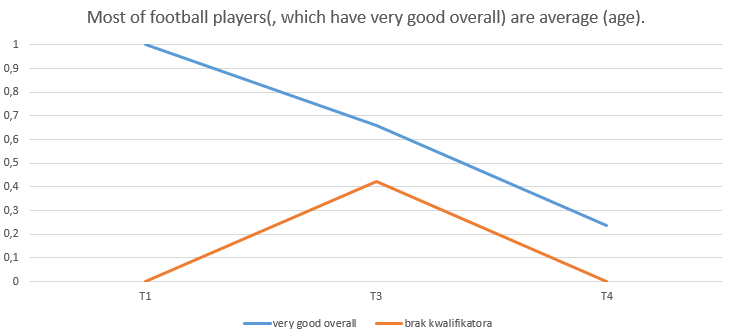
\includegraphics[width=0.9\textwidth]{ex/2a.png}
		\caption{Porównanie miar jakości T1, T3 i T4 w zależności od obecności kwalifikatora, sumaryzator złożony z jednej etykiety.}
		\label{wykresex2a}
	\end{figure}
	
	\begin{table}[h!]
		\centering
		\begin{tabular} {c c c}
			\hline
			\textbf{Miara} & \textbf{very good overall} & \textbf{brak kwalifikatora} \\ [0.5ex] 
			\hline	
			\hline 
			T1	&1&	0\\
			T3	&0,658&	0,421\\
			T4	&0,237&	0\\			
			\hline			
		\end{tabular}
		\caption{Miary $T_1$, $T_3$ oraz $T_4$ w zależności od obecności kwalifikatora. }
		\label{tabelaex2a}
	\end{table}

	W drugim przypadku, kwantyfikatorem była etykieta "Almost none", sumaryzatorem etykiety "slow and bad finishing", a kwalifikatorem "weak curve". Wartości miar jakości $T_2$ oraz $T_5 - T_8$ były stałe i wynosiły: $T_2 = 0.692, T_5 = 0.5, T_6 = 0.836, T_7 = 0,890$ oraz $T_8 = 0.245$. Miary $T_9$ - $T_{11}$ zależą od kwalifikatora, więc nie były brane pod uwagę w porównaniu.	
	
	
	\begin{figure}[h!]
		\centering
		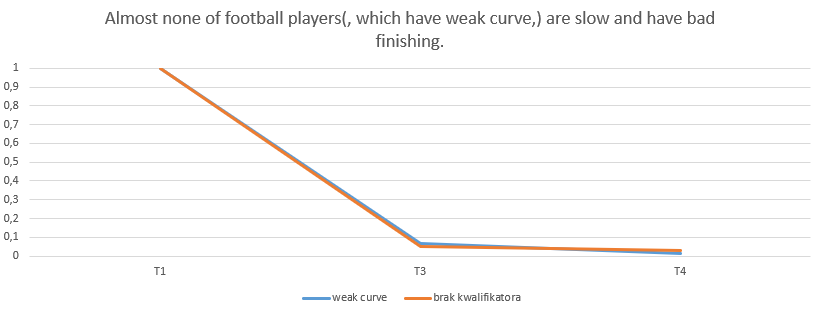
\includegraphics[width=0.9\textwidth]{ex/2b.png}
		\caption{Porównanie miar jakości T1, T3 i T4 w zależności od obecności kwalifikatora, sumaryzator złożony z dwóch etykiet.}
		\label{wykresex2b}
	\end{figure}
	
	\begin{table}[h!]
		\centering
		\begin{tabular} {c c c}
			\hline
			\textbf{Miara} & \textbf{weak curve} & \textbf{brak kwalifikatora} \\ [0.5ex] 
			\hline	
			\hline 
			T1	& 1 &	1 \\
			T3	& 0,068 &	0,053\\
			T4	& 0,014 &	0,029 \\			
			\hline			
		\end{tabular}
		\caption{Miary $T_1$, $T_3$ oraz $T_4$ w zależności od obecności kwalifikatora. }
		\label{tabelaex2b}
	\end{table}

	\newpage
	\subsection{Porównanie podsumowań z sumaryzatorem oraz złączeniem kilku sumaryzatorów}
	W tej sekcji pokażemy porównanie 3 różnych zdań ze stałym kwantyfikatorem oraz kwalifikatorem. 
	Wybrane przez nas sumaryzatory wyglądały następująco:
	\begin{itemize}
		\item $S_1$ - Average finishing
		\item $S_2$ - Average shot power
		\item $S_3$ - Average finishing AND average shot power
	\end{itemize}

	Podobnie, jak w poprzednich sekcjach, niektóre z miar jakości miały stałe wartości i wynosiły: $ T_6 = 0.671, T_7 = 0.726$  oraz $T_9 = T_{10} = T_{11} = 0$ - brak kwalifikatora.

	\begin{figure}[h!]
		\centering
		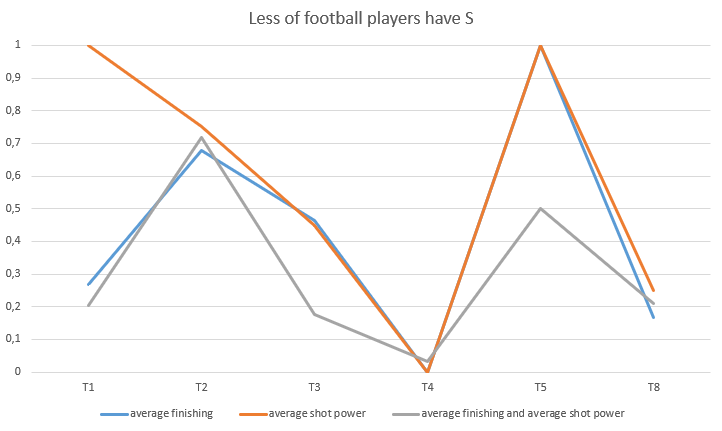
\includegraphics[width=0.9\textwidth]{ex/3a.png}
		\caption{Porównanie miar jakości w zależności od sumaryzatora.}
		\label{wykresex3a}
	\end{figure}
	
	\begin{table}[h!]
		\centering
		\begin{tabular} {c c c c}
			\hline
			\textbf{Miara} & \textbf{average finishing} & \textbf{average shot power} & \textbf{AND} \\ [0.5ex] 
			\hline	
			\hline 
			T1 & 0,268 &	1     & 0,203 \\
			T2 & 0,677 &	0,753 & 0,718 \\
			T3 & 0,465 &    0,449 & 0,177 \\
			T4 & 0     &	0	  & 0,032 \\
			T5 & 1     &	1     & 0,5   \\
			T8 & 0,167 &	0,25  & 0,209 \\
					
			\hline			
		\end{tabular}
		\caption{Porównanie miar jakości w zależności od sumaryzatora. }
		\label{tabelaex3a}
	\end{table}

	\newpage
	\subsection{Porównanie miary degree of truth dla różnych typów zdań wielopodmiotowych}
	
	W tym badaniu sprawdzaliśmy, jakie są wyniki miary jakości Degree of Truth w zależności od wyboru formy podsumowania wielopodmiotowego.
	Dla tego eksperymentu:
	\begin{itemize}
		\item S = 'very high'
		\item W = 'average (age)'
		\item P1 - Goalkeepers (bramkarze)
		\item P2 - Midfielders (pomocnicy)
	\end{itemize}
	Poniżej przedstawiamy wygenerowane zdania w każdej z form.
	\begin{enumerate}
		\item Almost all of goalkeepers in comparision to midfielders are very high.
		\item Almost all of goalkeepers in comparision to those midfielders, who are average (age), are very high.
		\item Almost all of those goalkeepers, who are average (age), in comparision to midfielders, are very high.
		\item More goalkeepers than midfielders are very high.
	\end{enumerate}
	
	\begin{figure}[h!]
		\centering
		\includegraphics[width=0.9\textwidth]{ex/4.png}
		\caption{Wykres porównujący miary Degree of Truth w zależności od formy podsumowania wielopodmiotowego.}
		\label{wykresex4a}
	\end{figure}
	
	\begin{table}[h!]
		\centering
		\begin{tabular} {c c}
			\hline
			\textbf{Forma podsumowania} & \textbf{$T_1$} \\ [0.5ex] 
			\hline	
			\hline 
			1 forma & 1 \\ 
			2 forma & 1 \\ 
			3 forma & 0.21006 \\
			4 forma & 0.79485 \\     
			\hline			
		\end{tabular}
		\caption{Porównanie miary Degree of Truth w zależności od formy podsumowania wielopodmiotowego. }
		\label{tabelaex4a}
	\end{table}
	
	\section{Dyskusja} % Dyskusja
	\subsection{Wpływ kwantyfikatora na miary jakości w zdaniach jednopodmiotowych}
	Wartość miary $T_1$ była różna od 0 tylko dla dwóch kwantyfikatorów na wykresie \ref{wykresex1a} oraz tylko dla jednego na wykresie \ref{wykresex1b}. Tam, gdzie wartość wynosiła 1, wiemy, że to podsumowanie jest dopasowane do danego kwantyfikatora. 
	
	W przypadku miar $T_6$ oraz $T_7$, które opisują nieprecyzyjność oraz liczność kwantyfikatora, wartości oscylowały w okolicach wartości 0.8, czyli dosyć wysokie wartości. Dla pierwszego przypadku, tylko dla kwantyfikatora \textsl{More than 3000} wartość tych miar była bardzo niska i wyniosła ok. 0,164. 
	
	Pozostałe miary, tj. $T_2 - T_5, T_8 - T_{11}$ nie zmieniały swoich wartości, gdyż te miary nie zależą od wybranego kwantyfikatora.
	
	\subsection{Wpływ kwalifikatora na miary jakości w zdaniach jednopodmiotowych}
	W tym eksperymencie widać znaczącą różnicę miary $T_1$ w pierwszym przykładzie - dla zdania z kwalifikatorem wartość $T_1$ wyniosła 1, a dla zdania bez kwalifikatora - 0. Również miary $T_3$ oraz $T_4$ znacznie się od siebie różniły.
	
	W drugim przykładzie, wszystkie miary $T_1$, $T_3$ oraz $T_4$ miały bardzo podobne wartości. $T_1 = 1$, natomiast $T_3$ oraz $T_4$ były bliskie 0.
	
	Miary pozostałe, które nie zostały uwzględnione w wynikach były stałe, gdyż nie zależały od wyboru kwalifikatora, natomiast miary $T_9 - T_{11}$ nie były badane, gdyż bez kwalifikatora nie da się ich obliczyć.
	
	\subsection{Porównanie podsumowań z sumaryzatorem oraz złączeniem kilku sumaryzatorów}
	W tym badaniu największą różnicę możemy zauważyć dla miary $T_1$ - dla sumaryzatora "average shot power" wartość wyniosła 1, natomiast dla sumaryzatora "average finishing" oraz ich złączenia wyniki były bliskie wartości 0.2. 
	
	Miara $T_2$, określająca precyzyjność sumaryzatora największą wartość osiągnęła dla sumaryzatora $S_2$, lecz złączenie dwóch sumaryzatorów ($S_3$) dało lepszy wynik niż sumaryzator $S_1$. 
	
	Wartości miary $T_3$ były bardzo podobne dla sumaryzatorów $S_1$ i $S_2$, lecz dla ich złączenia wartość drastycznie spadła. Wartość miary $T_4$ jest bliska zeru dla wszystkich sumaryzatorów.	
	 
	Wartość miary $T_5$ spadła z wartości 1 dla pojedynczych sumaryzatorów do wartości 0.5 dla ich złączenia, gdyż ta miara jest zależna od ilości zbiorów rozmytych, na które składa się sumaryzator.
	
	Miara $T_8$ dla wszystkich sumaryzatorów zawsze wyniosła około 0.2.
	
	\subsection{Porównanie miary degree of truth dla różnych typów zdań wielopodmiotowych}
	
	W przypadku podsumowań wielopodmiotowych, liczymy tylko miarę Degree of Truth. Jak można zauważyć na wykresie \ref{wykresex4a} oraz tabeli \ref{tabelaex4a}, wartości dla pierwszej i drugiej formy wyniosły 1, ale dla 3 formy już ok. 0.21. Dla 4 formy wynik wyniósł ok. 0.79.
	
	\section{Wnioski}
	\begin{itemize}
		\item Lingwistyczne podsumowania baz danych znacznie przyspieszają analizę danych z wieloma atrybutami poprzez generowanie informacji zrozumiałych dla człowieka. 
		\item Im większa ilość krotek w bazie, tym lepsze będą podsumowania bazy danych.
		\item Najlepiej jest dobrać więcej wąskich przedziałów funkcji przynależności, tak, aby można było uzyskać najlepsze wyniki.
		\item Miara $T_1$ jest najważniejsza w porównaniu wygenerowanych podsumowań, lecz lepiej jest porównać również wyniki innych miar jakości
		\item Etykiety powinny się na siebie nakładać, aby uniknąć pustych obszarów w dziedzinie.
		\item Część z wygenerowanych przez program komunikatów była do przewidzenia przed wygenerowaniem podsumowań. Teraz jednak możemy stwierdzić to za pomocą formalnej i statystycznej miary.
	\end{itemize}

	\newpage
	\begin{thebibliography} {0}
		\bibitem{anbook} Niewiadomski, Adam. Methods for the Linguistic Summarization of Data: Applications of Fuzzy Sets and Their Extensions. Akademicka Oficyna Wydawnicza EXIT. Warszawa, 2008. ISBN 978-83-60434-40-6
		\bibitem{anbookpl} Niewiadomski, Adam. Zbiory rozmyte typu 2. Zastosowania w reprezentowaniu informacji. Akademicka Oficyna Wydawnicza EXIT. Warszawa, 2019. ISBN 978-83-7837-595-1
		\bibitem{anarticle30} Pozyskiwanie wiedzy z relacyjnych baz danych: wielopodmiotowe podsumowania lingwistyczne. [online]  [dostęp 04.06.2020]
		http://cejsh.icm.edu.pl/
		cejsh/element/bwmeta1.element.desklight-48b6e678-8bdb-4a2b-ab79-
		77a76631b2e5/c/30.pdf
		\bibitem{tresc} Treść zadania 2. [online] [dostęp 04.06.2020] https://ftims.edu.p.lodz.pl/
		pluginfile.php/132360/mod\_resource/content/6/ksr-projekt2-2019.pdf
		\bibitem{baza} Źródło bazy danych zawodników z gry FIFA 20. [online] [dostęp 04.06.2020] https://www.kaggle.com/stefanoleone992/fifa-20-complete-player-dataset
		\bibitem{kul} https://pracownik.kul.pl/files/31717/public/Funkcje\_przynaleznosci.pdf [dostęp 07.05.2020]
		\bibitem{funkcje} http://ii.uwb.edu.pl/rudnicki/wp-content/uploads/2016/02/P07.pdf [dostęp 08.05.2020]
	\end{thebibliography}
\end{document}
